\subsection*{\center{General description of work}}The area of research in which the thesis is complex and involves different areas of work, in particular, creation of intelligent systems. Scope intelligent systems are vast, for example, in the Institute Starting (India) E. Jubilson and P. Dhanavantini conducting research of intellectual systems of processing of user requests in the field of telecommunications, and the University of Hannover (Germany) R. Bruns and George Dankel develop intelligent systems for query processing in service of rescue to reduce response time to incident. In Saint-Petersburg state University (SPSU) under the leadership of V. I. Zolotarev assesses the effectiveness of an information service support in the computer center of SPBU. In Singapore S. Fu and P. Leong made the analysis of the effectiveness of large companies support and the possibility of some processes automation (IT~-- information technology).\par
Research in the field of intelligent systems to improve the efficiency of it services companies are also leaders in the it industry: HP Company \footnote{The project \url{https://en.wikipedia.org/wiki/HP_OpenView}} and IBM \footnote{The project \url{http://www.ibm.com/smarterplanet/us/en/ibmwatson/}}. For example, the famous multi-purpose intelligent system IBM Watson, the development and study of which the unit under the guidance of Professor A. Goel.  \par   In order that the system can work with user requests, it must \quoted{understand} the language in which they are made. Such problems are studied in the field of natural language processing. For example, this is the GATE approach \footnote{The project \url{https://gate.ac.uk/}}, which is actively developing at the University of Sheffield (UK) under the direction of G. Callaghan, L. Moffat and S. Szaz. Another direction~--- this semantic search, research in this area has also actively conducted at the University of Sheffield, in particular, the developed approach Mimir, which implements the search functionality on the principle "search and discovery". For search of solutions in accordance with user requests in such systems, ontologies are used, for example, the widely used approach proposed by S. Dey and A. James from University of California (USA) based on the use of trees of tags in the ontology. \par
To give to the intelligent flexibility is needed to enable it to carry out logical reasoning. One of the leading organizations in this line of research is a OpenCog consortium \footnote{The project \url{http://opencog.org/}} (USA). These works leads by Ben Hertzel (Chairman of Artificial General Intelligence Society and OpenCog Foundation)~--- one of the world leaders in the field of artificial intelligence. Research in the field of machine logic is also underway in the framework of The projectа NARS \footnote{The project \url{https://sites.google.com/site/narswang/}} under the guidance of Temple University Professor (USA) Pey Wong. \par 

\newcommand{\actuality}{\underline{\textbf{The relevance topic.}}}
\newcommand{\aim}{{\textbf{Goal}}}
\newcommand{\tasks}{{\textbf{tasks}}}
\newcommand{\scope}{{\textbf{Field of study}}}
\newcommand{\subject}{{\textbf{The subject of the study is}}}
\newcommand{\methods}{{\textbf{Research methods}}}
\newcommand{\defpositions}{{\textbf{The main provisions submitted for~defense:}}}
\newcommand{\novelty}{{\textbf{Scientific novelty}}}
\newcommand{\influence}{{\textbf{Practical significance.}}}
\newcommand{\reliability}{{\textbf{Reliability}}}
\newcommand{\probation}{{\textbf{Probe of the work.}}}
\newcommand{\contribution}{{\textbf{Personal contribution.}}}
\newcommand{\publications}{{\textbf{Publication.}}}

{\aim} of the thesis is to develop an intelligent system of improving the efficiency of it operations-enterprise services. \par
{\scope}~--- systems development of databases and knowledge.\par
{\subject}  is the registration process and resolving of problem situations arising in infrastructure of the enterprise.\par
{\methods}~--- theoretical methods: simulation, theory of knowledge bases in the field of artificial intelligence; special techniques: system modeling; experimental methods: the method of observation, experimentation.\par 
To achieve this goal we solved the following problems and {\tasks}:
\begin{enumerate}
  \item To analyze the system of knowledge management in supporting the information infrastructure of the enterprise;
  \item To design and build a model of the problem-oriented system of knowledge management for decision-making and optimization of the processes of registration, analysis and processing of user requests in the service area of the information infrastructure of the enterprise;
  \item On the basis of built model to develop the architecture and prototype of an intelligent system of improving the efficiency of it operations-enterprise services;
  \item To hold the testing of the prototype on test data.
\end{enumerate}

\defpositions
\begin{enumerate}
  \item The analysis results of the database management systems knowledge of the it support infrastructure;
  \item The constructed model of the problem-oriented system of knowledge management and optimization of processes of user requests in the service area of enterprise's infrastructure;
  \item Created a prototype software implementation of the problem-oriented model system of knowledge management and the optimization processing of user requests in the service areas of it infrastructure enterprise;
  \item The results of testing of a prototype problem-oriented control system in the control examples.
\end{enumerate}

\novelty\ the conducted research are the following:
\begin{enumerate}
  \item On the basis of generalization of the model of thinking developed by M. Minsky created a simulation model of the problem-oriented system of management, decision-making in the field of maintenance of it infrastructure of enterprise;
  \item Investigated the possibilities of using models of thinking in relation to the service area of the information infrastructure of the enterprise;
  \item The new schema, and the original storage method for a model of thinking that is more efficient than standard ways storage (such as a relational database) was shown;
  \item On the basis of generalization of the Minsky thinking model was created the architecture service system of the information infrastructure of the enterprise and a software prototype of this system.
\end{enumerate}

\influence\ The system developed in the framework of the thesis, has considerable practical. The idea of work affected by the production problems in the it industry, with which the author faced daily in the process of resolving various incidents arising from the activities of technical support \icl~--- one of the largest backbone enterprises of the it industry of the Tatarstan Republic. Therefore it was necessary to develop a deep understanding of a particular subject area, to select an acceptable software solution, to receive a practical application in the organization of informational support of it-infrastructure specific enterprise. \par
\reliability\ scientific results and developed practical recommendations are based on correct formulation and General private the considered problems, using well-known fundamental theoretical provisions, sufficient volume of data used in statistical modelling, and a wide experimental material used for numerical estimates of achievable quality indicators. \par 
Research conducted in the thesis correspond to the passport of the specialty 05.13.11~--- Mathematical and software of computers machines, complexes and computer networks, the mapping is shown in the table \ref{ResearchDescription}.
\renewcommand\tablename{Table} 
\begin{longtable}{|p{8cm}|p{8cm}|}
 \caption[A comparison of the areas of research stipulated in the specialty 05.13.11, and the results obtained in the thesis]{Mapping directions research provided by specialty 05.13.11, and the results obtained in the thesis}\label{ResearchDescription} \\ 
 \hline
 
 \multicolumn{1}{|c|}{\textbf{The research direction}} & \multicolumn{1}{c|}{\textbf{The result of work}}  \\ \hline 
\endfirsthead
\multicolumn{2}{c}%
{{\bfseries \tablename\ \thetable{} -- continued}} \\
\hline \multicolumn{1}{|c|}{\textbf{The research direction}} &
\multicolumn{1}{c|}{\textbf{The result of work}}  \\ \hline 
\endhead
\endfoot

\hline \hline
\endlastfoot
\hline
   Programming languages and system programming, semantics of programs & Developed a semantic model of the knowledge storage organization \\
   \hline
  The database management system and knowledge & Developed a prototype Thinking Understanding (TU) storage systems knowledge and decision-making in the sphere of support of the it infrastructure of the enterprise, which was tested on synthetic data\\
   \hline
   Models and methods of designing programs and software systems for parallel and distributed data processing languages and tools 
for parallel programming & The developed method of parallel processing of expert information and the opportunity for learning with the help of the prototype TU \\
  \end{longtable}


\probation\
 The main results of the thesis were presented at the following conferences:
\begin{itemize}
	\item Tenth 

youth scientific school-conference \quoted{Lobachevskii reading~---2011}. Kazan, October 31st,~--~November 4th 2011;
	\item  International conference"3rd World Conference on Information Technology (WCIT-2012)". Barcelona, 14~--~16 November 2012, Spain; 
	\item II International conference «Artificial intelligence and natural language (AINL-2013)». Saint Petersburg, May 17~--~18 2013 ;
	\item VI International scientific-practical 

conference «E-Kazan 2014». Kazan, April 22~--~24 2014;
	\item XVI All-Russian scientific conference "Digital libraries: 

advanced methods and technologies, digital collections (RCDL-2014)». Dubna, October 13~--~16 2014; 
	\item Seminars on software engineering "All-Kazan Software Engineering Seminar (AKSES-2015)". Kazan, 9 April 2015;
	\item International conference "Agents and multi-agent systems: technologies and applications (AMSTA-2015)". Sorento, 17~--~19 June 2015, Italy.
\end{itemize}Practical approbation of results was carried out during unloading of the incidents of registration system queries, technical support of it infrastructurestructure \icl. The expected was the result in 51\% (the percentage of resolved issues, set by the user), but the result achieved in 30\% we believe acceptable, as it significantly increases the effective resolution problem queries. \par
\contribution\ The author conducted the analysis of user requests and classified them; built a model of the target region and identified opportunities to optimize processes. Data for the study (discharge from registration systems of user requests \iclshort) have been obtained the help of A. V. Krechov.  Together with M. O. by Talanov the author has created a basic architecture of the system. The author has developed system components tested systems on experimental data and fine-tune its work. \par
\publications\ The main results on the topic of the thesis is presented in 10 publications \cite{Lobachevskii, WCIT-2012,  ISGZ, IJSE-1, IJSE-2, RCDL-2014, AMSTA-2015, VAK-1, EB-1, EB-2}, of which articles \cite{RCDL-2014, AMSTA-2015} indexed in Scopus and included in the list of journals of higher attestation Commission of the Russian Federation, article \cite{AMSTA-2015} also indexed in the database Web of Science, work \cite{VAK-1} published in the journal of the higher attestation Commission of the Russian Federation, article \cite{ISGZ} indexed in the database of Russian science citation index, works \cite{Lobachevskii, WCIT-2012, ISGZ} published in the proceedings of international and national conferences, articles \cite{IJSE-1, IJSE-2} published in the international journal "International Journal of Synthetic Emotions"\,, which is included in Association for Computing Machinery. \par
In work \cite{Lobachevskii} A. S. Toshev suggested the original idea of the automatic construction of applications. The article \cite{WCIT-2012} A. S. Toshev developed a software complex, M. O. Talanov suggested the idea, and V. A. Krekhov provided test data from the registration system requests the technical support of it infrastructure \icl. In work \cite{ISGZ} A. S. Toshev proposed and implemented the architecture of an intelligent agent, M. O. Talanov set the task of checking the results of implementation of this approach. In articles \cite{IJSE-1, IJSE-2} A. S. Toshev performed the validation of the model proposed by M. O. Talanov. In the work \cite{RCDL-2014} A. S. Toshev implemented the model. In the article \cite{ AMSTA-2015} A. S. Toshev completed the refinement of the model of thinking, M. O. Talanov set the task of giving versatility system. In the article \cite{VAK-1} A. S. Toshev analyzed the results of the system of registration of requests of technical support of it infrastructure \icl\ and hypothesized about the possibility of automating the permissions part of the query. In the works \cite{EB-1, EB-2} A. S. Toshev conducted development and testing model, M. O. Talanov has developed a basic conceptual idea. \par


 % The characteristics of the structure in the introduction and in the abstract no different (GOST Р 7.0.11, items 5.3.1 and 9.2.1), because its downloaded from the same external file, but must first be allocating some parameters

%The thesis work was performed with the support of grants ...

%\underline{\textbf{The volume and structure of work.}} The thesis consists of~introduction, four chapters, conclusions and~application. Full 

%scope of the thesis \textbf{ХХХ}~pages with~\textbf{ХХ}~drawings and~5~tables. The bibliography contains \textbf{ХХX}~name.

%\newpage
\subsection*{The content of the work}
In \textbf{introduction} it justifies urgency of studies conducted in the framework of the thesis; the General characteristics work and analysis of research in the field of maintenance of information infrastructure of the company; reviewed and based on the identified growth publication activity in the subject area (according to Scopus) the urgency of the research conducted. \par

\textbf{First Chapter} the thesis is devoted to the formulation and review of intelligent systems recording and analysing problem situations that arise in it the infrastructure of the enterprise.
The Chapter begins with descriptions of models of the theory of mass service (TMS) for services involved in Troubleshooting the problem situations arising in the it infrastructure of the enterprise. In picture \ref{img:mass_service} presents a model of a Queuing system in which the following designations are used: $\lambda$ --- the intensity of the incoming stream;  
$\alpha$ --- the share of applications for which the waiting time in the queue exceeds $max(T_q)$;       
$\mu$ --- the reciprocal of the average time spent by the application agent;
$n$ --- the number of agents;
$T_q$ --- time orders in the queue in hours;
$SLA$ --- the level of service or the share of applications for which the time in the queue does not exceed $max(T_q)$, $SLA=1-\alpha$;
 $T_p$ --- the time of satisfaction of the application;
 $\alpha_n$ --- the number of applications;
 $T_{qp}=T_q+T_p$ --- the time of passage of applications through the system;
 $S(\mu)= \frac{R_p}{\mu} $ --- the average cost of performing a single application;
 $R_p$ --- the average cost of a working hour of a specialist (displayed next).

  
\begin{figure} [h] 
  \center
  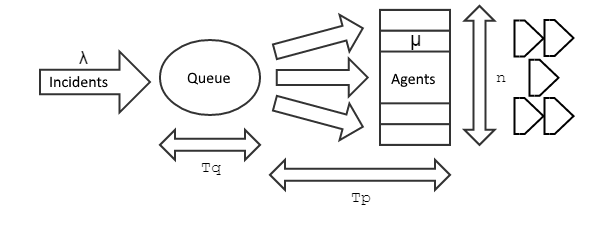
\includegraphics [scale=0.8] {mass_service-eng}
  \caption{The model of queueing system.} 
  \label{img:mass_service}  
\end{figure}
There are several approaches for solving tasks of TMO: 
\begin{itemize}
	\item An analytical solution for the simplest systems, which allows to express $T_q (t)$ through $\lambda$, $\mu$ и $n$;
	\item The solution using a simulation approach, where a histogram of $T_q (t)$, against which to measure the adequacy of $n$ for ensuring of SLA;
	\item Solution using the econometric approach, which is suitable for systems with a sufficiently large $n$. In such systems it is possible to estimate $T_q (t)$ according to the statistics.
\end{itemize} \par
Based on the combination of the Erlang formulas, Engset model and Polyachek model ~--~CHinchin built the formula for the solution of tasks of TMO on the basis of the analytical approach by finding the probability distribution for $T_{qp}$. The main task of the this work is the prediction of necessary resources to maximize $SLA$ ($SLA=1-\alpha$). In Chapter 1 of the thesis we consider the problem of minimizing $T_{qp}$, $S(\mu)$ and dynamic resource allocation. Based on the statistics collected in the company \icl,~ was calculated the following ratio $T_{qp}=47,9$ при $n=6$; $SLA=0,82$; $\alpha=0,18$;  $\alpha_n=2920$.  \par
Chapter 1 also presented comparative analysis of the registration systems and resolve problem situations; establishes the basic requirements for intelligent systems and  analysis of problem situations in the it field. One important element of such systems is natural language processing, therefore, in this Chapter comparative analysis of methods and software packages word processing. \par
The analysis has used the following tools natural language processing: Open NLP\footnote{The project \url{http://opennlp.apache.org}}, Relex\footnote{The project \url{http://opencog.org}}, StanfordParser\footnote{The project \url{http://nlp.stanford.edu/software/lex-parser.shtml}}. Evaluation of quality of functioning of these funds were held using the metrics presented in table \ref{Metrics}, and the results are shown in figure \ref{img:ParserCompare}. As can be seen, the best result in all three metrics showed the system Relex, she was selected as the primary means of natural language processing. \par

\newpage

\begin{figure} [h] 
  \center
  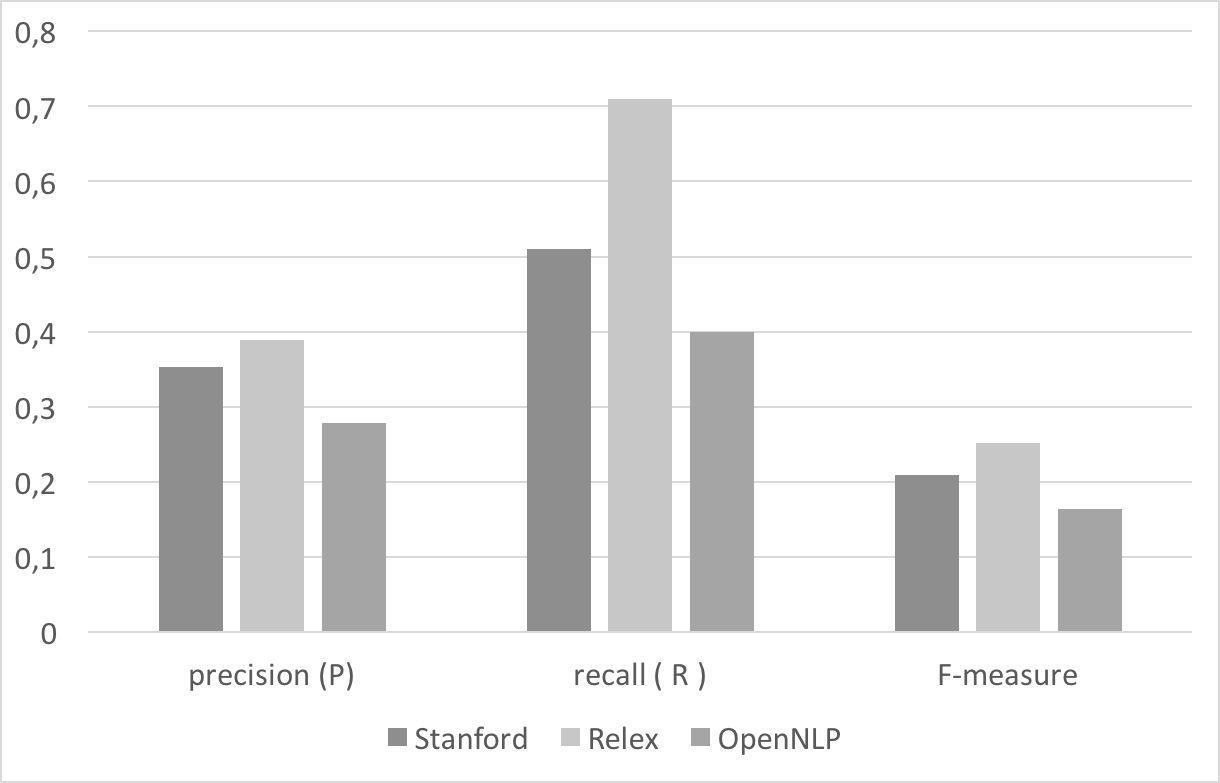
\includegraphics [scale=0.7] {ParserCompare}
  \caption{Results analysis of the means natural language processing} 
  \label{img:ParserCompare}  
\end{figure}


\renewcommand\tablename{Table} 
\begin{longtable}{|p{2cm}|p{4cm}|p{8cm}|}
 \caption[The metrics table]{The metrics table}\label{Metrics} \\ 
 \hline
 \multicolumn{1}{|c|}{\textbf{Metric}} & \multicolumn{1}{c|}{\textbf{Description}} & \multicolumn{1}{c|}{\textbf{Formula}} \\ \hline 
\endfirsthead
\multicolumn{2}{c}%
{{\bfseries \tablename\ \thetable{} -- continue}} \\
\hline\multicolumn{1}{|c|}{\textbf{Metric}} & \multicolumn{1}{c|}{\textbf{Description}} & \multicolumn{1}{c|}{\textbf{Formula}}  \\ \hline 
\endhead
\endfoot

\hline \hline
\endlastfoot
   \hline
Precision	& Precision & 
$$ 
P=\frac{tp}{tp+fp},
$$ where $P$~--- precision, $tp$~---  successfully processed words, $fp$~--- false successful \\
 \hline
Recall	& Sensitivity & 
$$ 
R=\frac{tp}{tp+fn},
$$ where $R$~--- recall, $tp$~--- successfully processed words, $fn$~--- false failure \\
 \hline
$F$	& $F$~--- measure (the performance) & 
$$ 
F=\frac{P*R}{P+R},
$$ where $P$~--- precision, $R$~--- recall.   \\

 
\end{longtable}
In addition, in Chapter 1 the analysis of existing software systems of automation in the field support of information infrastructure of the enterprise: HP Open View\footnote{\url{https://ru.wikipedia.org/wiki/HP_OpenView}}, ServiceNOW\footnote{\url{http://www.servicenow.com/}}, IBM Watson\footnote{\url{http://www.ibm.com/smarterplanet/us/en/ibmwatson/}}.Installed all of the above not meet the full set of necessary requirements listed in the introduction. Table \ref{Comparsion} contains summary information for the considered systems~--- indicates the presence or absence of a particular feature. As can be seen, none of the considered solutions is not able conduct logical reasoning. The most developed to date software system is a complex IBM Watson.
\renewcommand\tablename{Table} 
\begin{longtable}{|p{6cm}|p{0.5cm}|p{0.5cm}|p{0.5cm}|}
 \caption[Comparative analysis of existing software systems.]{Comparative analysis of existing software systems.}\label{Comparsion} \\ 
 \hline
 
 \multicolumn{1}{|c|}{\textbf{Comparative paragraph}} & \multicolumn{1}{c|}{\textbf{HP Open View}} & \multicolumn{1}{c|}{\textbf{ServiceNOW}} & \multicolumn{1}{c|}{\textbf{IBM Watson}} \\ \hline 
\endfirsthead
\multicolumn{2}{c}%
{{\bfseries \tablename\ \thetable{} -- continue}} \\
\hline \multicolumn{1}{|c|}{\textbf{Comparative paragraph}} & \multicolumn{1}{c|}{\textbf{HP Open View}} & \multicolumn{1}{c|}{\textbf{ServiceNOW}} & \multicolumn{1}{c|}{\textbf{IBM Watson}}  \\ \hline 
\endhead
\endfoot

\hline \hline
\endlastfoot
\hline
   Monitoring & Yes & Yes & Yes \\
   \hline
   Registration of incidents & Yes & Yes & Yes\\
   \hline
   Systems management & Yes & No & No \\
   \hline 
   Create the processing chain (Workflow) of incendent & Yes & Yes & No \\
   \hline 
   Understanding and the formalization of natural language queries & No & No & Yes \\
   \hline 
   Finding solutions & No & No & Yes \\
   \hline 
   Application of solutions & No & No & No \\
   \hline
   Training & No & No & Yes \\
   \hline
   Ability to conduct logical reasoning: generalization, specialization, synonymous search & No & No & No \\
   
\end{longtable}



%=================
%===Second chapter
%=================

\textbf{The Second Chapter} пsanctified the construction of a model 

intelligent decision-making system for recording and analysing problem situations in the it infrastructure of the enterprise. Consider three fundamental approach to solving the problem:
 \begin{itemize}
	\item model Menta 0.1, built using decision trees;
	\item модель Menta 0.3, built using genetic algorithms;
	\item model TU 1.0, based on the model of thinking of Marvin Minsky.
\end{itemize} \par
Note the model built on the basis of neural networks (supporting training), was rejected at the preliminary assessment stage, as it makes large performance requirements that in turn leads to high cost. Next, each model is described in detail.

\textbf{Model of Menta 0.1, built using decision trees}, was one of the first that was tested. When building the model used the following 

Components: processing natural language queries; the search for a solution; applying the solution. \par
The system is designed to execute simple commands for example, the "add field to form". In General, the system is characterized by the following algorithm:
\begin{enumerate}
	\item obtaining and formalization of the request;
	\item finding solutions with the help of trees decision-making;
	\item changing the model of application format OWL;
	\item generate and compile the application.
\end{enumerate} \par
In the result of experiments revealed the absence of error tolerance, input: grammatical and meaningful. For example, the input file is not relate to a software system model which contained in the knowledge base; the system solver only worked in the framework of the one programme; there was no learning function. \par

\textbf{Model of Menta 0.3, built using genetic algorithms}.In this model, compared to 
the previous module has been added to the logic for evaluating solutions and the module of genetic algorithms to generate solutions. In the model of Menta 0.3 was fulfilled the following basic Components of the future final model: acceptance criteria (Acceptance Criteria); How-To~--- storage solutions analyzed problems; the data format is OWL; the use of logical calculations to validate the solution. System 0.3 Menta contain, as a Component of part, model the target application (as Menta 0.1) and a list of solutions to certain problems (How-To) found earlier. With the help of genetic algorithm the model was built the solution, checked it with a logic engine NARS\footnote{\url{http://www.cogsci.indiana.edu/farg/peiwang/papers.html}} on the criteria defined by the user. From the point of view of genetic algorithms, this check is~--- function selection of individuals from generation.  \par
In the result of the experiments identified the following problems: lack of training; lack of natural language processing; after testing it turned out that the list of criteria the solution of the requirement of the user (rules) almost describe the necessary decision (the one that should be found) that was invalid. \par


\textbf{The TU model 1.0, model-based thinking Marvin Minsky}, was built using well-known theories of Marvin Minsky\footnote{\url{https://en.wikipedia.org/wiki/The_Emotion_Machine}}, retained the following main conceptual elements previous models and has demonstrated its viability in the control examples: Acceptance Criteria; training; finding and applying solutions; no natural language processing. This model is more versatile and is a high level architecture of the query processing (thinking) where Components are best in terms of functionality Components of the previous systems. Implemented model is called TU, and demonstrated its viability in the control examples (from English "Thinking andUnderstanding\"~~--- «thinking and understanding»). \par

One of the main Components of the system TU is a triplet \triplet\ (later \tripletshort), schematic representation of which is presented in figure \ref{img:csw}. The critic responds, the Selector selects the resource, a Way of thinking does work.
\begin{figure} [h] 
  \center
  \includegraphics [scale=1.0] {CSW-en}
  \caption{\tripletshort} 
  \label{img:csw}  
\end{figure}


\emph{Critic} is a switch that is triggered under certain events. For example, "turn on the light, and the pupils are narrowed", "burned and pulled hand." Critic is activated only when enough circumstances. At the same time can be activated several Critic. For example, man solves a difficult task, there is activation of many Critic: to calculate, to clarify the technical details. In addition, the parallel may Critic is activated to control the activity level of reporting needed rest.\par
\emph{Selector} deals with the selection of required resources which, for example, can be: a Critic, a way of thinking. \par
\emph{Way of thinking}~--- this method of solving the problem. It can be challenging and, for example, can activate other Critic. So, thinking about the problem, the specialist understands that it is necessary to consider all possible combinations, and then he decides look for a turnkey solution: maybe someone has already considered all the possible combinations, and you can use it. Here, the "search solutions" is Critic inside the way of thinking "search solution".\par

On the picture \ref{img:csw_ex} presents an expanded model of work \tripletshort. Critic activates the selector, which returns the resource way of thinking (the circles marked with a variety of resources: Criticи, selectors, ways of thinking \etc). Last in turn, you can activate a new Criticа or to perform certain actions. For example, there was a problem related to lack of access, so, we need to run the utility to grant rights to the user. Under the resource here refers to knowledge from knowledge base: Critics, selectors, ways of thinking, ready-made solution. \par 
If activated a lot of Critic, the problem needs to be clarified, otherwise the uncertainty will be too high. If the problem is very similar to the already analysed, it is possible to act and to judge by analogy. \par
\begin{figure} [h] 
  \center
  \includegraphics [scale=0.6] {CSW_EX_en}
  \caption{\tripletshort\ in the context of resources} 
  \label{img:csw_ex}  
\end{figure}
Another important part of the theory of Minsky are the levels of thinking. This concept distributes the activity of thinking between 6 levels: the higher the level, the stronger the activity. The Table \ref{ThinkingLevelDescription} the description of levels of thinking with examples. \par
The study of models of thinking was completed and was made conclusions, the main of which are as follows. 

\newpage
\begin{longtable}{|p{5cm}|p{10cm}|}
 \caption[Description of the six levels of thinking inherent in the model Minsky.]{Description of the six levels of thinking inherent in the model Minsky.}\label{ThinkingLevelDescription} \\ 
 \hline
 
 \multicolumn{1}{|c|}{\textbf{Level}} & \multicolumn{1}{c|}{\textbf{Description}}  \\ \hline 
\endfirsthead
\multicolumn{2}{c}%
{{\bfseries \tablename\ \thetable{} -- continue}} \\
\hline \multicolumn{1}{|c|}{\textbf{Level}} & \multicolumn{1}{c|}{\textbf{Description}}   \\ \hline 
\endhead
\endfoot

\hline \hline
\endlastfoot
\hline
  Instinctive level & instinctive reactions Occur (congenital). For example, the knee-jerk reaction. The General formula for this level can be expressed as "if ... then do so" \\
  \hline Learned level & Use the accumulated knowledge, i.e. the knowledge that a person trained in the course of life. For example, to cross the road on green light. The General formula for this level can be described as "if ... then do so" \\
  \hline Deliberative level & Thinking using reasoning. For example, if you cross the road on green light, you can make it in time. At this level compares the effects of several solutions and select the optimal. The General formula for this level can be expressed as "if ... then to make so then be it" \\
  \hline
Reflective level & Reasoning based on the analysis of past events. For example, "the last time I ran on the blinking green and almost got hit by a car" \\

  \hline
  Self-reflective level & Build a specific model, which is an estimation of the actions. For example, "my decision not to go to the meeting was incorrect, since I missed so many chances, I was distracted" \\
  \hline
  Self-Conscious level & Evaluation of their actions from the point of view of higher ideals and assessments of others. For example, "what will my friends think? And how would my hero react?" \\
   
\end{longtable}

For the software expert system is very important to have the ability to think and reason, for example, to proceed by analogy. A lot of typical queries, the queries differ only in the parameters. For example, one of them is a request "please install Office, Antivirus» \etc\ For expert systems it is important to be able to abstract specialized solution recipes. For example, the system learned to resolve the incident "Please install Firefox"\comma\ to obstreperous the incident to the extent "Please install browser"\comma\ the system will be able the same the way to fix the problem "Please install Chrome"\comma\ same as concept "Firefox"\ and "Chrome"\ linked through the concept of "Browser". \par
After consideration of multiple models was chosen as model of thinking Marvin Minsky, as it best matches the target region support of it infrastructure of the enterprise. Based on the approach Minsky built a model of the system that implements the core functions: teaching, understanding of the incident, search solutions, application solutions. 


%=================
%===3rd chapter
%=================
In \textbf{the third Chapter} describes the architecture and implementation of the system based on the model Thinking Understanding (TU).
The architecture is a module. The main system Components described in the Table \ref{MainComponents}. The system can operate in learning mode and in the mode of elimination of problematic situations. 
\begin{longtable}{|p{7cm}|p{8cm}|}
 \caption[The main Components of the system Thinking Understanding]{The main Components of the system Thinking Understanding}\label{MainComponents} \\ 
 \hline
 
 \multicolumn{1}{|c|}{\textbf{Component}} & \multicolumn{1}{c|}{\textbf{Description}}  \\ \hline 
\endfirsthead
\multicolumn{2}{c}%
{{\bfseries \tablename\ \thetable{} -- continue}} \\
\hline \multicolumn{1}{|c|}{\textbf{Component}} &
\multicolumn{1}{c|}{\textbf{Description}}  \\ \hline 
\endhead

\endfoot

\hline \hline
\endlastfoot
\hline
   TU Webservice & The main Component of the interaction with external systems, including user \\
   \hline
   CoreService & The system core contains the basic classes\\
   \hline
   DataService & Component of work with the data \\
   \hline 
   Reasoner & Component of probabilistic logic \\
   \hline 
   ClientAgent & Component of run scripts on the target machine \\
   \hline 
   MessageBus & Data bus for the system \\
    
\end{longtable}
Chapter 3 provides a detailed Description of all Component and Component under. For a better understanding of the Description of the mechanism the interaction Component and the overall usage scenario of the system.
%Each paragraph, subparagraph and list recorded with indentation (GOST 2.105-95, 4.1.8)

\begin{enumerate}
	\item A request comes in from user: 
	"User had received wrong application. User has ordered Wordfinder Business Economical. However she received wrong version, she received Wordfinder Tehcnical instead of Business Economical. Please assist"\ («The user got the wrong app. The user has ordered app "Wordfinder. Business license"\,, but got the wrong version,~--- "Wordfinder. Technical version." Please help»);
	\item Component GoalManger (Manager of goals) sets the target system HelpUser (To help the user);
	\item Main Component of Thinking Life Cycle (later TLC) activates a set of Components Critic (Critic), tied to this goal (HelpUser); 
	\item Activates Component PreliminaryAnnorator (Pre-processor), which parses the request, conducting a spelling correction and pre analysis;
	\item Component KnowledgeBaseAnnotator (analysis using accumulated knowledge) creates a semantic network and a reference to it;
	\item Component Critic (Critic), tie it to a goal HelpUser on a Reflexive level, runs WayToThink (Way of thinking) ProblemSolving (To resolve problem situation) with the aim: ResolveIncident;
	\item Component Critic on Reflexive level selects WayToThink KnowingHow (Search prescription solutions);
	\begin{enumerate}
	\item Run in parallel all Components of a class Critic, who is bound to the target ResolveIncident (To solve the problem), in this case they are DirectInstruction (direct instructions), ProblemWithDesiredState (problem with desired state), ProblemWithoutDesiredState (the problem is no desired state);
	\item Component Selector (Selector) chooses among all results, the most probable result. In this case they will be Problem Description with desired state (The problem with the desired state);
	\item Component KnowingHow saves the options Selector;
	\item Component Simulation (Modelling) WayToThink with parameters "to create a model of the current situation" creates the conception of the current situation (CurrentState), the concept of the user concept software;
	\item Component Reformulation WayToThink (Component of add), using the results of the previous step, synthesizes the artifacts, which is not enough to get out CurrentState DesiredState (The desired state), as it is not explicitly specified. WayToThink runs Critic thoughts to find the root of the problem. He finds CurrentState (the current status)~--- Wordfinder Tehcnical and DesiredState (the condition that the user needs)~--- Wordfinder Business Economical;
	\item Reflexive Critic assess the state of the system~--- at which step it is and if the goal is not achieved, then start another WayToThink, for example, DirectInstruction;
	\item Component Critic Solution Generator (Component of Solution Generator) runs KnowingHow WayToThink, ExtensiveSearch (The search for a solution);
	\item Component Selector selects the most probable way of thinking. In this case will ExtensiveSearch that will find solutions that allow the system to be the desired user as (DesiredState), if this is not possible, the system initiates communication with the user. 
 \end{enumerate}
	 \item Reflective Critic checks the status of the system. If the Goal is reached, the user is sent a response informing about it.
	 \item In this step, activated Components class Critic at the conscious level, which store information about the costs of the solution.
  \end{enumerate}\par
For the system created the unique data model~--- TU Knowledge, which combines OWL and graph database. The OWL that appeared to structure the information in the web, has gained wide use in many data schemas, as it gave the opportunity for more extended descriptions of the relationships between. 

%=================
%===4 chapter
%=================
In \textbf{4th chapter} the results of evaluating the performance of model obtained on the basis of the conducted experiments.
Tests were conducted to perform a comparison with the work of the specialist-human. Was selected checklist of queries user (incident). We compared the speed of incident resolution. The main time in the survey of the expert is spent on communication. The table \ref{HumanComparison} the results of the comparison. Tests were performed on the computer Intel Core i7 1700 MHz, 8GB RAM, 256 GB SSD, FreeBSD. From results show that the system works as well or better than the technical support specialist.
\begin{longtable}{|p{12cm}|p{2cm}|p{2cm}|}
 \caption[The results of the comparison with the work of a specialist]{The results of the comparison with the work of a specialist}\label{HumanComparison} \\ 
 \hline
 
 \multicolumn{1}{|c|}{\textbf{The incident}} & \multicolumn{1}{c|}{\textbf{TSS1 (.мс)}} & \multicolumn{1}{c|}{\textbf{TU (.мс)}}  \\ \hline 
\endfirsthead
\multicolumn{2}{c}%
{{\bfseries \tablename\ \thetable{} -- continued}} \\
\hline
\multicolumn{1}{|c|}{\textbf{The incident}} & \multicolumn{1}{c|}{\textbf{TSS1 (.мс)}} & \multicolumn{1}{c|}{\textbf{TU (.мс)}}  \\ \hline 
\endhead

\endfoot

\hline \hline
\endlastfoot
\hline
  Tense is kind of concept~(Time~--- is the concept) & 15000 & 385 \\
  
  \hline
  Please install Firefox~(Install Firefox)   & 9000 & 859 \\
  \hline
  Browser is an object~(Browser~--- this is an object)   & 20000 & 400 \\
  \hline
  Firefox is a browser~(Firefox~--- this is the browser)   & 5000 & 659  \\
  \hline
  Install is an action~(Install~--- this is an action)   & 8000 & 486 \\
  \hline
  User miss Internet Explorer 8~(The user does not have Internet Explorer 8).     & 10000 & 10589 \\
  \hline
  User needs document portal update~(The user must update the documents)    & 15000 & 16543 \\
  \hline
  Add new alias Host name on host that alias is wanted to: hrportal.lalala.biz IP address on host that alias is wanted to: 322.223.333.22 Wanted Alias:    webadviser.lalala.net~(Please add 

a new link to hrportal.lalala.biz through 322.223.333.22)    & 10000 & 18432  \\ 
  \hline
  Outlook Web Access (CCC)~--- 403~--- Forbidden: Access is denied~(There is no access to Outlook Web Access (CCC)). & 15000 & 10342\\ 
  \hline
  PP2C~--- Cisco IP communicator. Please see if you can fix the problem with the ip phone, it's stuck on configuring ip + sometimes Server error rejected: Security etc~(PP2C~--- Communicator Cisco IP. Please help to fix the problem with SP-phone, it gets stuck during the configuration and sometimes shows the error "Security")  & 13000 & 12343 \\ 
   
  \end{longtable}
  The indicators presented in the introduction, has acquired the following values $T_qp$=32,9 with n=8; SLA=0,96; $\alpha$=0,04;  $\alpha_n$=2920. 

%=================
%===Conclusion
%=================
In \textbf{Conclusion} of theses are the main conclusions of the work:
%% According to GOST standart Р 7.0.11-2011:
%% 5.3.3 In the conclusion of the thesis present the results of the completed studies, recommendations and prospects for further development of the topic.
%% 9.2.3 In the conclusion of the dissertation present the results of this research, recommendations and prospects for further development of the topic.

Solved the following tasks and produced the following results.
\begin{enumerate}
  \item Was created a model of problem-oriented knowledge management system in the field of maintenance of information infrastructure of the enterprise on the basis of generalization of the model of thinking;
  \item Presented a new data model for the thought patterns of the original and the method of their storage more efficient compared to classical databases that use a relational approach;
  \item Performed original research patterns of thinking in the field of maintenance of information infrastructure of the enterprise;
  \item Based on the model developed in the thesis, created the system architecture and its prototype; 
  \item The system developed in this paper, includes innovative methods and algorithms for decision support, uses a generalized model of thinking Minsky;
  \item Presents visualization of the structure of the region remote support infrastructure.
\end{enumerate}

Presented in the thesis model of thinking, its architecture and implementation are unique~--- at this time it is the only implementation of the Minsky model of thinking. \par
The system developed in the thesis, is highly specialized and suitable for other areas where required knowledge base, for example, when the medical diagnosis in order to reject the false diagnoses. \par
In the diagnosis of problems you can train the system information about the components of the car and problems associated with them, the signs of these problems and their solutions. \par
Work is performed partially at the expense of the subsidy allocated to Kazan Federal University for the state assignment in the sphere of scientific activities, projects 1.2368.2017, «Budget 17-97».






 

%\newpage
\renewcommand{\refname}{\large Author's publications on dissertation topic}

%\insertbiblioauthor                          % Plug-Bib-base
\insertbiblioalleng

